%!TEX root = "../../DA_GUI.tex"

%	--------------------------------------------------------
% 	Aufbau der Benutzeroberfläche
%	--------------------------------------------------------

\chapter{Elemente der Benutzeroberfläche}
In diesem Kapitel wird der grundlegende Aufbau aller Fenster und Benutzeroberflächen von C Compact beschrieben - sowohl die konzeptuelle Konstruktion als auch die Implementierung.
\section{Das Konzept}
Die Erscheinung und Bedienung von C Compact folgt durchgehend der grundlegenden Idee, eine einfach und intuitiv zu bedienende Entwichlungsumgebung zu schaffen. Das bedeutet, Features möglichst Zielgruppenorientiert zu integrieren und überflüssige Funktionen zu vermeiden. Durch besondere Rücksicht auf Vollständigkeit und logische Bedienvorgänge haben wir ein durchgängig logisches Bedienerlebnis angestrebt.
Konkret haben wir uns dabei an folgende Ŕegeln gehalten:
\begin{itemize}
\item Das Erscheinen von Elementen in der Benutzeroberfläche soll logisch begründbar und verständlich vermittelbar sein
\item Funktionen, die im FSST-Unterricht der ersten und zweiten Klassen wahrscheinlich nicht benötigt werden, werden vermieden oder sind standardmäßig deaktiviert; Bedienelemente werden also auf das wesentlichste reduziert
\item Wir sind der Meinung, dass eine intuitiv zu bedinenede Oberfläche nicht durch Animationen und große Symbole erzeilt werden kann, sondern durch einfache, bereits bekannte Konzepte. So sind in C Compact bekannte Elemente wie beispielsweise eine Menüleiste mit gewohnten Datei- und Dokumentoperationen zu finden (Siehe Kapitel \ref{sec:gui-main-menu}).
%TODO reference GUImain
\end{itemize}

\subsection{Daraus resultierende Einschränkungen}
Durch diese Reduktion der gesamten Oberfläche ist C Compact auf einen bestimmten Zweck, also die Ausbildung, beschränkt. Das sehen wir allerdings nicht als Nachteil, sondern als besondere Stärke. Mit C Compact wollen wir eine Entwicklungsumgebung schaffen, die Anfänger nicht überfordert und ihnen hilft, sich auf das wesentliche zu konzentrieren.
Das Konzept einer anfängerfreundlichen Entwichlungsumgebung ist mit dem Aufbau einer Umgebung für die professionelle Entwicklung nicht vereinbar. C Compact soll aber auf späteres Arbeiten mit komplexeren Programmen vorbereiten. Schüler, die ihre erste Programmiersprache mit C Compact erlernen, kennen bereits den Umgang mit einem Debugger und haben ein tieferes verständnis für den Ablauf von Programmen.

%TODO add window desc. for launcher, quest seleter, package selecter
\section{Elemente und Fenster Der Benutzeroberfläche}
Neben dem Hauptfenster, das den Kern der Benutzeroberfläche darstellt, gibt es eine Reihe von kleineren Aktionsfenster, Dialogen und Einstellungsfenstern, die zum reibungslosen Ablauf bei der Bedienung von C Comapct beitragen. Das Hauptfenster selbst wird in Kapitel \ref{sec:gui-main} beschrieben.

\subsection{Launcher}
\label{sec:win-launcher}
...

\subsection{Einstellung der Sprache}
\label{sec:win-lang}
Wenn C Compact zum ersten Mal gestartet wird, wird zu allererst dieses fenster angezeigt. Der Benutzer wird gebeten, eine Sprache zu wählen. Später kann die Sprache über das Menü ,,Datei'' im Hauptfenster (Siehe Kapitel \ref{sec:gui-main-menu-file}) geändert werden. Die Änderungen werden erst wirksam, wenn der Benutzer die neue Sprache mit ,,OK'' bestätigt. Dann wird C Compact neu gestartet.
%TODO ref translations, Sprache

\begin{figure}[htp]
\centering
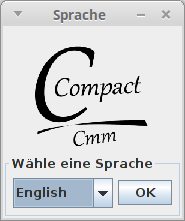
\includegraphics[width=0.3\textwidth]{./media/images/gui/elements/Bildschirmfoto-Sprache.png}
\caption{Auswahl der Sprache}
\label{fig:win-lang}
\end{figure}

Dieses Fenster ist in der Klasse \textbf{GUILanguage} im Package \textbf{at.jku.ssw.cmm.gui.properties} implementiert. 

\subsection{Allgemeine Einstellungen}
\label{sec:win-set}
Dieses Fenster enthält allgemeine Optionen zum Haupfenster der Benutzeroberfläche. Es kann im Menü des Hauptfensters unter ,,Datei'' -> ,,Einstelungen'' aufgerufen werden (Siehe Kapitel \ref{sec:gui-main-menu-file}). Änderungen an den Einstellungen werden sofort wirksam (ausgenommen sind Änderungen an der Schriftgröße von Dokumenten). Da C Compact beim Ändern dieser Einstellungen nicht neu gestartet werden muss, sind diese Optionen und die Spracheinstellungen in zwei unterschiedliche Fenster aufgeteilt.
%TODO ref GUImainSettings

\begin{figure}[htp]
\centering
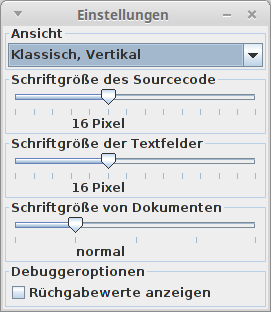
\includegraphics[width=0.4\textwidth]{./media/images/gui/elements/Bildschirmfoto-Einstellungen.png}
\caption{Einstellungsfenster}
\label{fig:win-set}
\end{figure}

Im Einstellungsfenster können folgende Optionen verändert werden:
\begin{enumerate}
\item \textbf{Ansicht:} Ändert den Aufbau des Hauptfensters. Elemente werden je nach gewähltem Layout unterschiedlich angeordnet. Siehe Kapitel \ref{sec:gui-main-left-ord}.
\item \textbf{Schriftgröße des Sourcecode:} Ändert die Schriftgröße des Textfeldes für den Sourcecode im Hauptfenster. Siehe Kapitel \ref{sec:gui-main-left-code}.
\item \textbf{Schriftgröße der Textfelder:} Ändert die Schriftgröße der Textfelder für Ein- und Ausgabedaten im Hauptfenster. Siehe Kapitel \ref{sec:gui-main-left-io}.
\item \textbf{Schriftgröße von Dokumenten:} Dokumente, wie etwa Beschreibungstexte von Fehlern, können mit unterschiedlichen Textgrößen angezeigt werden. Da die Schriftgröße beim Initialisieren der Textfelder festgelegt wird, betrifft die Einstellung immer nur die Dokumente, die in Zukunft geöffnet werden.
%TODO ref Fehlerdokumente
\item \textbf{Rückgabewerte anzeigen:} Hier kann eine Funktion des Debuggers aktiviert werden, die noch nicht ausgereift und auch nicht immer hilfreich ist: Wenn das Programm aus einer Funktion zurückspringt und in die Aufrufzeile einen Rückgabewert übergibt, wird dieser in einem Popup dargestellt.
%TODO Absatz nochmal lesen
%TODO ref popup
%TODO ref return popup
\end{enumerate}

Alle Klassen des Einstellungsfensters befinden sich im Package \textbf{at.jku.ssw.cmm.gui.properties}. Das Fenster selbst wird in der Klasse \textbf{GUIProperties} initialisiert, Listener für alle Schieberregler befinden sich in der Klasse \textbf{PropertiesSliderListener}. Die Combobox für das Layout der Benutzeroberfläche (Option 1) wird mit der Klasse \textbf{PropertiesComboListener} überwacht, die Checkbox für das Anzeigen von Rückgabewerten im Debugger ist mit dem ActionListener \textbf{PropertiesActionListener} verknüpft.

Beim Ändern der Schriftgröße werden zuerst die Einstellungen von C Compact verändert, dann werden die Schriftgrößen in den entsprechenden Elementen aktualisiert.
\begin{lstlisting}[language=JAVA]
@Override
public void stateChanged(ChangeEvent e) {
	JSlider slider = (JSlider)e.getSource();
	
	// Einstellungen aktualisieren
	main.getSettings().setCodeSize(GUIProperties.sliderPosToFont(slider.getValue()));
	
	// Schriftgrößen aktualisieren
	master.updateTextSize();
}
\end{lstlisting}

Tatsächlich wird beim aktuakisieren der Schriftgrößen einfach ein neuer Font mit der entsprechenden Größe aus dem bereits verwendeten Font abgeleitet und angewandt.
%TODO ref GUIleftPanel
\begin{lstlisting}[language=JAVA]
// Schriftart (font) ändern
this.jSourcePane.setFont(
	// Aktuellen Font ableiten
	this.jSourcePane.getFont().deriveFont(
		//Schriftgröße laut Einstellungen
		(float)this.main.getSettings().getCodeSize()
	)
);
\end{lstlisting}

Die Schriftgröße von Dokumenten wird, wie in Punkt 4 bereits erwähnt, beim laden des Dokumentes festgelegt.
%TODO ref Dokumente laden

\subsection{Über C Compact}
% !!! TODO mention SSW in credits !!!
Dieses Fenster enthält den Lizenztext von C Compact sowie die Namen der beteiligten Personen. Auch dieses Fenster kann im Menü der Entwicklungsumgebung aufgerufen werden (Menü siehe Kapitel \ref{sec:gui-main-menu-file}). Alle Bestandteile dieses Elementes befinden sich im Package \textbf{at.jku.ssw.cmm.gui.credits}:
\begin{itemize}
\item \textbf{Credits.java:} Initialisiert das Fenster und regelt sein Verhalten.
\item \textbf{credits.html:} Enthält den Lizenztext.
\item \textbf{credits.css:} Enthält formatierungsinformationen zum Lizenztext.
\end{itemize}
%TODO ref Dokumente laden

Die Resourcen sind im Package eingebunden und deshalb auch Teil der generierten JAR-Datei. Dadurch kann der Lizenztext nicht einfach verändert werden.

\begin{figure}[htp]
\centering
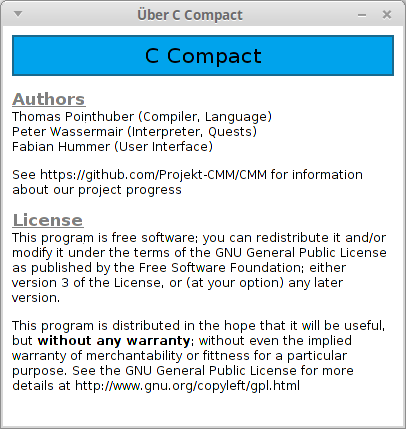
\includegraphics[width=0.4\textwidth]{./media/images/gui/elements/Bildschirmfoto-About.png}
\caption{Fenster mit Lizenztext}
\label{fig:win-about}
\end{figure}

\subsection{Questpacket auswählen}
...

\subsection{Quest auswählen}
...

\subsection{Profil erstellen}
... name eingeben ...

\subsection{Dialoge}
\label{sec:win-dialog}
In C Compact werden viele verschiedene Dialogfenster verwendet. Der Begriff Dialogfenster\footnote{http://de.wikipedia.org/wiki/Dialog\_(Benutzeroberfläche)} umfasst eine Reihe von unterschiedlichen Anwendungen, bei denen ein Fenster werwendet wird, um Informationen oder Befehle vom Benutzer einzuholen. Dialoge werden in C Compact beispielsweise verwendet, um zu fragen, ob eine Datei gespeichert werden soll (Abbildung \ref{fig:win-dialog}), oder um den Benutzer auf ein Problem aufmerksam zu machen. Swing enthält bereits einige Funktionen zum Erstellen von Dialogen\footnote{http://docs.oracle.com/javase/tutorial/uiswing/components/dialog.html}, anhand dieses Tutorials können einfache Dialoge sehr schnell erstellt werden.

\begin{figure}[htp]
\centering
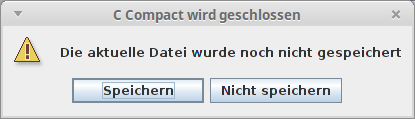
\includegraphics[width=0.4\textwidth]{./media/images/gui/elements/Bildschirmfoto-Dialog.png}
\caption{Ein einfacher Dialog}
\label{fig:win-dialog}
\end{figure}

\subsection{Dateimanager}
...

%TODO add information about info saved in profiles
\section{Einstellungen}
\label{sec:guimainsettings}
Für den Betrieb einer fortgeschrittenen Benutzeroberfläche ist es unerlässlich, diese anpassbar zu machen und Anpassungen des Benutzers zu speichern. Im Package \textbf{at.jku.ssw.cmm.gui.properites} befindet sich die Klasse \textbf{GUImainSettings}, die alle globalen Einstellungen überwacht. Diese Einstellungen umfassen:
\begin{itemize}
\item Die zuletzt geöffneten Dateien
\item Die gerade geöffnete Datei
\item Die zuletzt geöffneten Benutzerprofile
\item Das aktuell aktive Benutzerprofil
\item Die vom Benutzer gewählte Sprache
%TODO ref language
\item Einstellungen, die der Benutzer direkt verändern kann (Siehe Kapitel \ref{sec:win-set})
\begin{itemize}
\item Schriftgrößen
\item Layout der Benutzeroberfläche
\end{itemize}
\end{itemize}

Bevor das Hauptfenster der Entwicklungsumgebung gestartet werden kann, muss ein Objekt der Klasse \textbf{GUImainSettings} erstellt werden (Siehe dazu Kapitel \ref{sec:gui-main-impl}). Dabei werden die zuletzt gespeicherten Einstellungen geladen.

Die Einstellungen werden in der Datei \textbf{settings.xml} im Hauptverzeichnis von C Compact gespeichert. Bevor diese Datei ausgelesen wird, werden alle Einstellungsvariablen auf einen definierten Standardwert gesetzt. Sollten also bestimmte Informationen oder alle Einstellungen fehlen, werden die Standardwerte wieder hergestellt. Die Einstellungen werden beim Beenden von C Comapct gespeichert.

Die Einstellungsdatei \textbf{settings.xml} ist wie folgt aufgebaut:
\begin{lstlisting}[language=XML]
<?xml version="1.0" encoding="UTF-8" standalone="no"?>
<settings xmlns="settings.xml">
	<properties>
		<language>de</language>
		<codesize>16</codesize>
		<textsize>16</textsize>
		<varsize>16</varsize>
		<varoffset>0</varoffset>
		<descsize>0</descsize>
		<returnpopup>false</returnpopup>
	</properties>
	<lastfile>/home/fabian/Dokumente/C--/C_Compact_Alpha_1.4.5/examples/helloworld/helloworld.cmm</lastfile>
	<lastfile>/home/fabian/Dokumente/C--/C_Compact_Alpha_1.4.5/examples/random/random.cmm</lastfile>
	<lastfile>/home/fabian/Dokumente/C--/C_Compact_Alpha_1.4.5/examples/bubblesort/bubblesort.cmm</lastfile>
	<profile>/home/fabian/Dokumente/profile_Fabian</profile>
</settings>
\end{lstlisting}

Unter ,,properties'' befinden sich alle Parameter, die der Benutzer direkt einstellen kann (die Sprache bei den Spracheinstellungen, siehe Kapitel \ref{sec:win-lang} und alle anderen Einstellungen bei den allgemeinen Einstellungen, siehe Kapitel \ref{sec:win-set}). Darunter werden die zuletzt gewählten Profile aufgelistet (diese werden im Launcher angezeigt, siehe Kapitel \ref{sec:win-launcher}) und dann die zuletzt geöffneten Dateien (für die Auflistung im Menü der Entwicklungsumgebung, siehe Kapitel \ref{sec:gui-main-menu-ctrl}). Damit die Listen nicht zu lang werden, werden nur die letzten 10 geöffneten Dateien und die letzten 10 aktiven Profile gespeichert und angezeigt.
%TODO appendix: how to read XML file

\section{Anzeigen von internen Fehlern}
Unter Unständen kann es bei C Compact zu internen Fehlern kommen. Zu diesen Zählen auch Probleme die entstehen, wenn eine wichtige Datei gelöscht wurde oder nicht gefunden werden kann. Die in diesem Abschnitt beschriebenen Fehlermeldungen sollten nicht mit den Fehlerbeschreibungen des Debuggers verwechselt werden (Siehe Kapitel \ref{}). Wenn ein Fehler auftritt, wird die Fehlermeldung in Form eines Dialoges (Siehe Kapitel \ref{sec:win-dialog} angezeigt.
%TODO ref debugger error docs

\begin{figure}[htp]
\centering
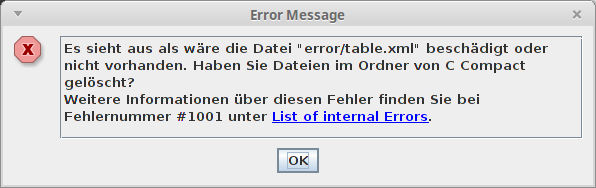
\includegraphics[width=0.5\textwidth]{./media/images/gui/elements/Bildschirmfoto-Error-Message.png}
\caption{Eine interne Fehlereldung}
\end{figure}

Jeder Fehler der auftreten kann hat eine eindeutige Fehlernummer, alle Fehler sind in der C Compact Projektwiki auf GitHub\footnote{https://github.com/Projekt-CMM/CMM/wiki/List-of-internal-error-numbers} aufgelistet. Eine Fehlernummer besteht immer aus 4 Zahlen; die erste gibt den Bereich an, in dem der Fehler aufgetreten ist.
%TODO keep this thable up to date
%TODO add references to different files/chapters
\def\arraystretch{1.6}
\begin{minipage}{14cm}
%\begin{table}[ht]
\begin{tabular}{l|l|l}
	Bereich&Nummer&Beschreibung\\
	\hline
	&1001&Datei \textbf{error/table.xml} fehlt\\
	\multirow{5}{15mm}{\begin{sideways}\parbox{35mm}{Dateien fehlen oder sind beschädigt}\end{sideways}}&1002&\multirow{2}{*}{Inhalt der Datei \textbf{error/table.xml} ist ungültig}\\
	&1003&\\
	&1011&Datei \textbf{error/style.css} fehlt oder ist beschädigt\\
	&1012&Inhalt der Datei \textbf{error/style.css} ist ungültig\\
	&1021&Fehlerbeschreibungsdokument nicht gefunden\\
	\hline
	&2001&Aktuelle Datei konnte nicht gespeichert werden\\
	\multirow{4}{15mm}{\begin{sideways}\parbox{25mm}{Dateien öffnen oder speichern}\end{sideways}}&2011&[inactive]\footnote{Dieser Fehler kann nicht mehr auftreten, da der zugehörige Bereich deaktiviert wurde}\\
	&2012&Datei konne nicht geöffnet werden\\
	&2013&Bibliothek konnte nicht gefunden werden\footnote{Dieser Fehler wird als Fehlermeldung im Debugger angezeigt. Die fehlernummer existiert nur formell}\\%TODO ref debugger error doc
	&2014&Datei \textbf{default.cmm} einer Quest konnte nicht geöffnet werden\\%TODO ref quest
	\hline
	%TODO add refs to quest testing
	&3001&Exception im Präprozessor\\
	\multirow{4}{15mm}{\begin{sideways}\parbox{25mm}{Testen einer Quest}\end{sideways}}&3002&[inactive]\footnote{Dieser Fehler kann nicht mehr auftreten} IOException im Präprozessor\\
	&3003&Unbekannter Fehler im Präprozessor\\
	&3004&Compiler wurde unerwartet beendet (Exception)\\
	&3005&Compiler durch Fehler im Sourcecode abgebrochen\\
	\hline
	\parbox{23mm}{Verbindungs- probleme}&9001&Fehler beim Drucken
\end{tabular}
%\caption{Interne Fehlernummern}
%\label{tab:int-err}
%\end{table}
\end{minipage}

%TODO TODO add some paragraphs about error window, error.xml, and so on

\section{Popups}
In C Compact gibt es mehrere Anwendungsfälle für Popup-Fenster. Popups werden verwendet, um weitere Informationen zu einem Array oder einem String in der Variablentabelle zu liefern und um Rückgabewerte von Funktionen zu visualisieren (dies ist allerdings optional, siehe auch \ref{sec:win-set} Dabei handelt es sich im Prinzip um kleine Anzeigeflächen, die ein Swing-Element enthält. Ein Popup wird ausgeblendet, sobald auf eine beliebige Fläche in einem Fenster von C Compact geklickt wird (der Event muss erfasst werden können).

\begin{figure}[htp]
\centering
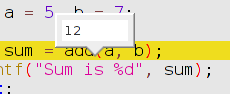
\includegraphics[width=0.4\textwidth]{./media/images/gui/popup/popup-example.png}
\caption{Ein Popup zeigt den Rückgabewert einer Funktion.}
\label{fig:popup-example}
\end{figure}

\subsection{Initialisierung eines Popups}
Die Popup-Funktionen selbst befinden sich in der Klasse \textbf{ImagePopup}. Zum Initialisieren werden aber die statischen Methoden in der Klasse \textbf{ComponentPopup} verwendet; diese Methoden übernehmen auch umständliche Positionsberechnungen für das Popup. Die Methode \textbf{createPopUp(...)} kann auch ohne das Parameter \glqq{}weight\grqq{} verwendet werden.
\begin{lstlisting}[language=JAVA]
public static void createPopUp( GUImain main, JComponent component, int x, int y, int w, int h, int orientation, double weight );
\end{lstlisting}

\begin{table}[h!]
\begin{tabular}{|ll|l|}
\hline 
GUImain & main  & Referenz auf das Hauptfenster, siehe \ref{sec:gui-main-impl} \\
\hline
JComponent & component & Das Swing-Element, das angezeigt werden soll \\
\hline
int & x & \multirow{2}{8cm}{Die Position, auf die das Popup zeigen soll} \\
int & y & \\
\hline 
int & w & \multirow{2}{8cm}{Höhe und Breite des Popups (Bezogen auf den äußeren Rand, \textbf{component} wird mit 5px Inset platziert)} \\
int & h & \\
\hline
int & orientation & Ausrichtung des Popups (siehe Unten) \\
\hline
double [optional] & weight & Position des Zeigers, Wert zwischen 0 und 1, Standard: 0.5\\
\hline
\end{tabular}
\caption{Parameter der Methode \textbf{createPopup(...)}}
\end{table}




